\documentclass[conference]{IEEEtran}
\IEEEoverridecommandlockouts
\usepackage{cite}
\usepackage{amsmath,amssymb,amsfonts}
\usepackage{algorithm}
\usepackage{algpseudocode}
\usepackage{graphicx}
\usepackage{textcomp}
\usepackage{xcolor}
\usepackage{booktabs}
\usepackage{multirow}
\usepackage{tikz}
\usetikzlibrary{arrows.meta,positioning,shapes.geometric,fit,calc}
\usepackage[hidelinks]{hyperref}
\graphicspath{{figures/}{../assets/}}

% ---- placeholders the author must fill in; each shows in red ----
\newcommand{\todo}[1]{\textcolor{red}{\textbf{[TODO: #1]}}}
\newcommand{\interpret}[1]{\textcolor{blue}{[INTERPRET: #1]}}
\newcommand{\maybeinput}[1]{\IfFileExists{#1.tex}{\input{#1}}{\todo{generated table \detokenize{#1} missing}}}
\def\BibTeX{{\rm B\kern-.05em{\sc i\kern-.025em b}\kern-.08em T\kern-.1667em\lower.7ex\hbox{E}\kern-.125em X}}

\begin{document}

\title{Kormat: Fine-Tuned Small-Language-Model Eligibility Screening with a From-Scratch KV Cache, Tiled Attention and Speculative Decoding on a CPU}

\author{\IEEEauthorblockN{Taha Ahmed}
\IEEEauthorblockA{Roll no.\ \todo{roll number}, Section \todo{section}\\
\todo{department / university}\\
\todo{email}}}

\maketitle

\begin{abstract}
% TODO-INTERPRET: fill numbers last, once Results are final.
We study criterion-level clinical-trial eligibility screening: given a patient note, a criterion type (inclusion or exclusion) and a criterion text, a model must return one of the expert label categories, including ``not enough information'' and ``not applicable'', together with supporting sentence IDs. We use the NCBI TrialGPT criterion annotations (1{,}015 annotations, 53 patients, patient-grouped 37/8/8 split, seed 42). A Qwen2.5-1.5B-Instruct model with a LoRA adapter, trained in a disclosed joint session on a shared GPU, is evaluated by us on a CPU laptop before and after adaptation. Beyond accuracy, we implement our own pre-allocated KV-cache decoder, a tiled online-softmax attention, and a greedy speculative decoder with a Qwen2.5-0.5B-Instruct draft, and wrap everything in a browser application. On the held-out test patients the adapted model reaches \todo{macro-F1 / accuracy}; the cache gives \todo{x} speed-up, tiled attention changes peak memory by \todo{y}, and speculative decoding gives \todo{z} with an acceptance rate of \todo{a}. We report these numbers with their limits.

\end{abstract}

\begin{IEEEkeywords}
clinical trial eligibility, criterion-level matching, LoRA, KV cache, online-softmax attention, speculative decoding, CPU inference
\end{IEEEkeywords}

\section{Introduction and Problem Statement}
\label{sec:intro}
Recruiting patients for clinical trials depends on reading long free-text notes against lists of inclusion and exclusion criteria. TrialGPT showed that a large language model can do this criterion by criterion, with explanations, close to expert accuracy~\cite{jin2024trialgpt}. That system relies on a closed, remote model, which is a cost and a privacy problem for patient text~\cite{nievas2023distilling}. This work asks a narrower and more practical question: \emph{how far can a small open model (1.5B parameters) adapted with parameter-efficient fine-tuning get on the criterion-level task, and what does it take to run it on a laptop CPU without a GPU?}

\textbf{Problem statement.} Input: a patient note split into numbered sentences, a criterion type (inclusion or exclusion) and a criterion text. Output: a label from the criterion type's own four-way set (included / not included / not enough information / not applicable for inclusion; excluded / not excluded / not enough information / not applicable for exclusion) and the list of supporting sentence IDs. Absent evidence is never treated as proof of eligibility or ineligibility. Any patient--trial verdict shown in our application is an aggregation by explicit rules, not a separately labelled ground truth.

\textbf{Contributions.}
\begin{enumerate}
\item A reproducible data pipeline over the mandated dataset with a patient-grouped split and leakage checks, excluding the dataset's GPT-4 predictions from all inputs (Sec.~\ref{sec:methods}).
\item A before/after evaluation of a LoRA-adapted Qwen2.5-1.5B-Instruct with accuracy, macro-F1, per-class scores, confusion matrices, evidence P/R/F1, split by criterion type (Sec.~\ref{sec:results}). The adapter itself was trained in a \emph{disclosed joint session} on a shared GPU with a classmate; evaluation and everything below are our own work.
\item Our own implementations of a pre-allocated KV-cache decoder, tiled online-softmax attention (Algorithm~\ref{alg:tiled}) and greedy speculative decoding (Algorithm~\ref{alg:spec}), each validated against the reference implementation and benchmarked on CPU.
\item A browser application, ``Kormat'', serving the pipeline with cited evidence and rule-based aggregation (Fig.~\ref{fig:app}).
\end{enumerate}
The remainder is organised as: related work (Sec.~\ref{sec:related}), methods (Sec.~\ref{sec:methods}), experimental setup (Sec.~\ref{sec:setup}), results (Sec.~\ref{sec:results}), limitations and conclusion.

\section{Related Work}
\label{sec:related}
\textbf{Clinical eligibility reasoning.} Early work framed patient-to-trial matching as retrieval, with test collections judged by medical professionals~\cite{koopman2016test}. TrialGPT moved to criterion-level reasoning with GPT-4, reporting 87.3\% criterion accuracy on the 1{,}015 expert-annotated pairs that form our dataset, and trial-level ranking~\cite{jin2024trialgpt}; its dependence on a closed model is the gap we address. Nievas et al.\ fine-tune open LLaMA models on GPT-4-generated synthetic data and report parity with proprietary models~\cite{nievas2023distilling}; we instead train only on expert labels and never use GPT-4 outputs as features.

\textbf{Architecture.} The Transformer~\cite{vaswani2017attention} is our attention reference. Grouped-query attention~\cite{ainslie2023gqa}, used in Qwen2.5~\cite{qwen2024qwen25}, shrinks the KV cache (Qwen2.5-1.5B: 12 query, 2 KV heads), which is what makes a CPU cache practical.

\textbf{Adaptation.} LoRA trains low-rank updates on frozen weights~\cite{hu2022lora}; QLoRA adds a 4-bit base~\cite{dettmers2023qlora}. For a 1.5B model, QLoRA's extra saving (about 2~GiB) does not justify its quantisation overhead, and full fine-tuning would need roughly 23~GiB (Sec.~\ref{sec:finetune}).

\textbf{Efficient inference.} The online normaliser~\cite{milakov2018online} and chunked attention~\cite{rabe2021selfattention} remove the need to materialise the $n\times n$ score matrix; FlashAttention~\cite{dao2022flashattention,dao2024flashattention2} makes it IO-aware on GPUs. Their speed-ups come from the GPU memory hierarchy, so we treat the CPU outcome as a hypothesis to measure, not a result to assume. Speculative decoding~\cite{leviathan2023speculative,chen2023speculative} lets a small draft propose tokens verified by the large model in one pass; its gain depends on draft acceptance and on cheap verification. PagedAttention~\cite{kwon2023pagedattention} and the scaling analysis of Pope et al.~\cite{pope2023scaling} address serving-scale KV management; our single-request app uses a contiguous pre-allocated cache instead.

\section{Materials and Methods}
\label{sec:methods}

\subsection{System overview}
Fig.~\ref{fig:pipeline} shows the pipeline. Components in the top row prepare data; the adapter was trained once in the joint session; everything in the lower row is ours and runs on CPU.
\begin{figure}[t]\centering
\resizebox{\columnwidth}{!}{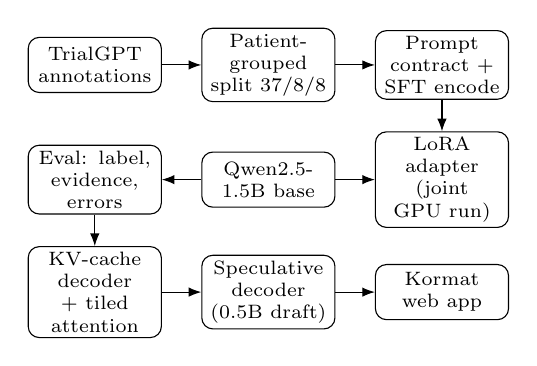
\begin{tikzpicture}[node distance=4mm and 5mm, box/.style={draw,rounded corners,align=center,font=\scriptsize,minimum height=7mm,inner sep=2pt,text width=1.55cm}, arr/.style={-{Latex[length=1.6mm]}}]
\node[box] (d) {TrialGPT annotations};
\node[box,right=of d] (s) {Patient-grouped split 37/8/8};
\node[box,right=of s] (p) {Prompt contract + SFT encode};
\node[box,below=of p] (l) {LoRA adapter (joint GPU run)};
\node[box,left=of l] (m) {Qwen2.5-1.5B base};
\node[box,left=of m] (e) {Eval: label, evidence, errors};
\node[box,below=of e] (k) {KV-cache decoder + tiled attention};
\node[box,right=of k] (sp) {Speculative decoder (0.5B draft)};
\node[box,right=of sp] (a) {Kormat web app};
\draw[arr] (d)--(s); \draw[arr] (s)--(p); \draw[arr] (p)--(l); \draw[arr] (m)--(l);
\draw[arr] (m)--(e); \draw[arr] (e)--(k); \draw[arr] (k)--(sp); \draw[arr] (sp)--(a);
\end{tikzpicture}
}
\caption{System pipeline: data preparation, adapted model, evaluation, own inference stack, application.}
\label{fig:pipeline}
\end{figure}

\subsection{Dataset and split}
\label{sec:dataset}
We use only the NCBI TrialGPT criterion annotations~\cite{trialgpt_criterion_annotations}: 1{,}015 criterion annotations for 53 patients, each with a patient description, criterion type and text, expert label and expert evidence sentence IDs. The dataset also contains GPT-4 predictions and explanations; these are never used as input or in evaluation. Unique patient IDs are sorted, shuffled with \texttt{numpy.random.default\_rng(42)}, and the first 37 go to training, the next 8 to validation and the last 8 to test; every annotation of a patient lies in exactly one split. The manifest is saved in \texttt{results/split\_manifest.json} and a leakage check asserts empty pairwise patient intersections. The test split was untouched until final evaluation.
\maybeinput{tables/data_stats} Fig.~\ref{fig:labels} shows the label distribution. % TODO-INTERPRET: split sizes, class imbalance
\begin{figure}[t]\centering
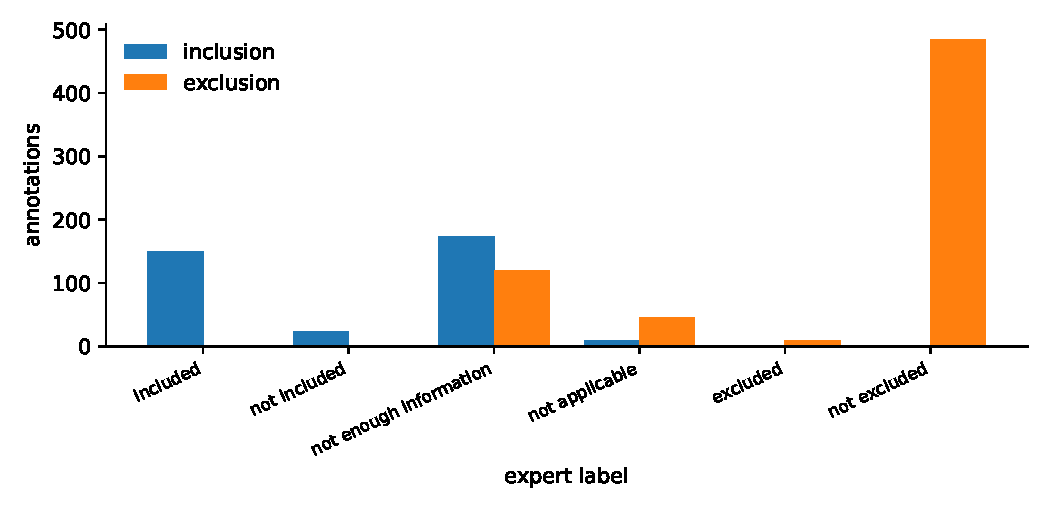
\includegraphics[width=\columnwidth]{figures/label_distribution.pdf}
\caption{Label distribution per criterion type and split.}
\label{fig:labels}
\end{figure}
% TODO-INTERPRET: Fig. labels: class imbalance, which classes are rare, consequence for macro-F1.

\subsection{Input/output processing and tokenization}
\label{sec:io}
Each patient note is split into numbered sentences following the dataset's sentence indexing. A single prompt contract (system message, numbered note, criterion type, criterion, allowed labels, JSON return format) is shared by training, evaluation, benchmarks and the app, so all see the identical string. The target is a JSON object \texttt{\{"label": ..., "evidence": [ids]\}}; the label set depends on criterion type and is never collapsed to yes/no. Text is tokenised with the Qwen2.5 tokenizer (151{,}936 tokens, identical for the 1.5B and 0.5B models) through the chat template. Training examples longer than 1{,}024 tokens are dropped, never cut mid-text, so no relevant evidence is silently removed.
\maybeinput{tables/token_lengths} Fig.~\ref{fig:toklen} shows the length distribution. % TODO-INTERPRET: number dropped per split, any evidence lost.
\begin{figure}[t]\centering
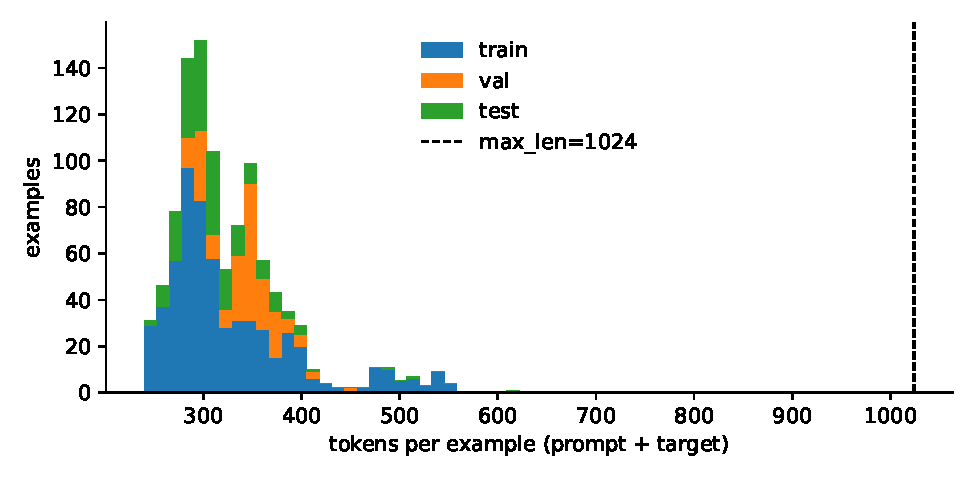
\includegraphics[width=\columnwidth]{figures/token_lengths.pdf}
\caption{Prompt length in tokens per split with the truncation threshold.}
\label{fig:toklen}
\end{figure}

\subsection{Model selection}
\label{sec:model}
Table~\ref{tab:models} compares four open-weight decoder candidates using the \texttt{config.json} files on the Hugging Face Hub (Llama-3.2-1B is gated, so its figures come from a public mirror). We chose Qwen2.5-1.5B-Instruct~\cite{qwen2024qwen25}: 28 layers, hidden size 1536, 12 query heads and 2 KV heads with head dimension 128, 32{,}768-token context, Apache-2.0, and a KV cache of 28{,}672 bytes per token in bf16, 6.9$\times$ smaller than the multi-head SmolLM2-1.7B. Qwen2.5-0.5B-Instruct shares its tokenizer (identical vocabulary, merges, special tokens, chat template; zero id mismatches on 50 test strings) and serves as the draft model. The base was fixed by the shared training run; we did not fine-tune the other candidates and make no claim that Qwen2.5 beats them.
\begin{table}[t]
\caption{Candidate open decoder models (config.json; memory by arithmetic, GiB).}
\label{tab:models}
\centering\scriptsize
\begin{tabular}{@{}lrrrr@{}}
\toprule
 & Qwen2.5-1.5B & Qwen3-1.7B & Llama-3.2-1B$^{\ast}$ & SmolLM2-1.7B \\
\midrule
Params (B) & 1.54 & 2.03$^{\dagger}$ & 1.24 & 1.71 \\
Layers & 28 & 28 & 16 & 24 \\
Hidden & 1536 & 2048 & 2048 & 2048 \\
Heads Q/KV & 12/2 & 16/8 & 32/8 & 32/32 \\
head\_dim & 128 & 128 & 64 & 64 \\
Vocab & 151,936 & 151,936 & 128,256 & 49,152 \\
Context & 32,768 & 40,960 & 131,072 & 8,192 \\
RoPE $\theta$ & $10^6$ & $10^6$ & $5\!\times\!10^5$ & 130,000 \\
Licence & Apache-2.0 & Apache-2.0 & Llama 3.2 & Apache-2.0 \\
fp32 / bf16 / 4-bit & 5.75/2.88/0.72 & 7.57/3.78/0.95 & 4.60/2.30/0.58 & 6.38/3.19/0.80 \\
KV B/token (bf16) & 28,672 & 114,688 & 32,768 & 196,608 \\
\bottomrule
\end{tabular}\\[2pt]
{\scriptsize $^{\ast}$ gated; values from public mirror. $^{\dagger}$ safetensors total incl.\ embeddings (card: 1.7B).}
\end{table}
% TODO-INTERPRET: Table models: GQA drives the KV-bytes column; why CPU RAM (15 GB) rules out larger caches; weights fit.

\subsection{Fine-tuning}
\label{sec:finetune}
\textbf{Disclosure.} The LoRA adapter was trained in a \emph{joint session} on a shared GPU with M.\ Ruhan Kamran (23i-0062) and published as \texttt{arceus1rk/eligitrace-qwen2.5-1.5b-lora}. We did not train it alone; we use it, and all evaluation, inference code and application are our own, run on a CPU laptop.

\textbf{Method choice.} For $N=1.54\times10^9$ parameters, full fine-tuning with mixed-precision AdamW needs about $16N\approx 23$~GiB for weights, gradients and optimiser state; LoRA~\cite{hu2022lora} with $r{=}16$ on $q,k,v,o,\mathrm{gate},\mathrm{up},\mathrm{down}$ trains 18{,}464{,}768 parameters (1.2\%), about 3.1~GiB in total; QLoRA~\cite{dettmers2023qlora} would reach about 1.0~GiB but adds quantisation overhead unnecessary at this size. Prompt-only is our ``before'' baseline.

\textbf{Configuration.} LoRA $r=16$, $\alpha=32$, dropout 0.05, 3 epochs, learning rate $2\times10^{-4}$ with cosine schedule, effective batch size 16, bf16. The training objective is next-token cross-entropy on the assistant JSON only (prompt tokens masked). % TODO-INTERPRET: confirm masking, warmup, seed, steps and curves from the shared run record; add training-curve figure in Results.

\subsection{Own KV-cache decoder}
\label{sec:kv}
We implement a per-layer pre-allocated buffer of shape (batch, KV heads, max length, head dim) and one integer \texttt{length}. Prefill writes all prompt keys and values (already RoPE-rotated) once; each decode step writes one position and attends to the view \texttt{buf[..., :length, :]}. Compared with concatenating tensors each step (copy cost $O(n)$ per token), a slice write is $O(1)$ in cache size, and rollback needed by speculative decoding only moves the integer (Fig.~\ref{fig:kv}). Cache size follows $2\cdot L\cdot n_{kv}\cdot d_h\cdot b$ bytes per token.
\begin{figure}[t]\centering
\resizebox{\columnwidth}{!}{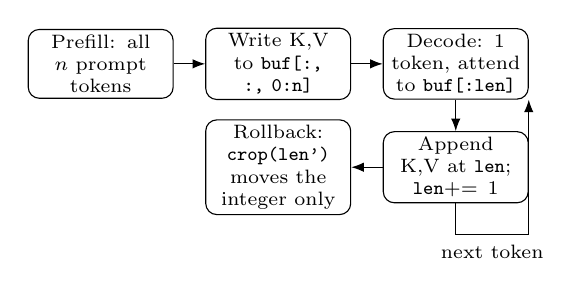
\begin{tikzpicture}[node distance=4mm, box/.style={draw,rounded corners,align=center,font=\scriptsize,minimum height=6.5mm,text width=1.7cm,inner sep=2pt}, arr/.style={-{Latex[length=1.6mm]}}]
\node[box] (pf) {Prefill: all $n$ prompt tokens};
\node[box,right=of pf] (w) {Write K,V to \texttt{buf[:, :, 0:n]}};
\node[box,right=of w] (dec) {Decode: 1 token, attend to \texttt{buf[:len]}};
\node[box,below=of dec] (app) {Append K,V at \texttt{len}; \texttt{len}$\mathrel{+}=1$};
\node[box,left=of app] (rb) {Rollback: \texttt{crop(len')} moves the integer only};
\draw[arr] (pf)--(w); \draw[arr] (w)--(dec); \draw[arr] (dec)--(app); \draw[arr] (app)--(rb);
\draw[arr] (app.south) -- ++(0,-4mm) -| node[pos=.25,below,font=\scriptsize]{next token} (dec.south east);
\end{tikzpicture}
}
\caption{Prefill and decode flow of the pre-allocated KV cache, with O(1) rollback.}
\label{fig:kv}
\end{figure}

\subsection{Tiled online-softmax attention}
\label{sec:attn}
For one head, $O=\mathrm{softmax}(QK^\top/\sqrt{d})V$. Following the online normaliser~\cite{milakov2018online} and its tiled use~\cite{rabe2021selfattention,dao2022flashattention}, we iterate over key blocks keeping a running row maximum $m$, normaliser $l$ and unnormalised output $O$ (Fig.~\ref{fig:tile}, Algorithm~\ref{alg:tiled}). The $L\times L$ matrix is never formed; only $B_q\times B_k$ tiles are. Accumulation is in fp32. Masks (causal, padding) are applied per tile; fully masked rows return zero and guard against $-\infty-(-\infty)$.
\begin{figure}[t]\centering
\resizebox{\columnwidth}{!}{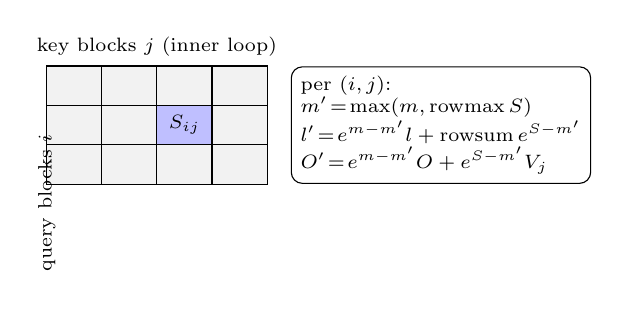
\begin{tikzpicture}[font=\scriptsize]
\foreach \i in {0,1,2} \foreach \j in {0,1,2,3} {
  \draw[fill=gray!10] (\j*0.7,-\i*0.5) rectangle ++(0.7,-0.5);
}
\draw[fill=blue!25] (1.4,-0.5) rectangle ++(0.7,-0.5);
\node at (1.75,-0.75) {$S_{ij}$};
\node[above] at (1.4,0) {key blocks $j$ (inner loop)};
\node[rotate=90,left] at (0,-0.75) {query blocks $i$};
\node[draw,rounded corners,align=left,right] at (3.1,-0.75) {per $(i,j)$:\\ $m'\!=\!\max(m,\mathrm{rowmax}\,S)$\\ $l'\!=\!e^{m-m'}l+\mathrm{rowsum}\,e^{S-m'}$\\ $O'\!=\!e^{m-m'}O+e^{S-m'}V_j$};
\end{tikzpicture}
}
\caption{Tile loop: for each query block, scan key blocks and update $(m,l,O)$.}
\label{fig:tile}
\end{figure}
\begin{algorithm}[t]
\caption{Tiled online-softmax attention (one head)}
\label{alg:tiled}
\begin{algorithmic}[1]
\Require $Q\in\mathbb{R}^{L_q\times d}$, $K,V\in\mathbb{R}^{L_k\times d}$, block sizes $B_q,B_k$, mask $M$
\For{each query block $Q_i$ ($B_q$ rows)}
  \State $m\gets -\infty,\; l\gets 0,\; O\gets 0$
  \For{each key block $(K_j,V_j)$}
    \State $S\gets Q_iK_j^\top/\sqrt{d}$; apply mask $M_{ij}$
    \State $m'\gets\max(m,\mathrm{rowmax}(S))$
    \State $P\gets \exp(S-m')$
    \State $l\gets e^{m-m'}\,l+\mathrm{rowsum}(P)$
    \State $O\gets e^{m-m'}\,O+PV_j$;\quad $m\gets m'$
  \EndFor
  \State output rows $O_i\gets O/l$
\EndFor
\end{algorithmic}
\end{algorithm}
We validate against the reference softmax attention (max absolute difference, and equality of generated tokens), see Sec.~\ref{sec:results}. Because the speed-ups reported for this family of methods come from GPU memory hierarchy~\cite{dao2022flashattention}, we expect memory savings on CPU but not necessarily speed-ups, and test this.

\subsection{Greedy speculative decoding}
\label{sec:spec}
We implement greedy speculative decoding~\cite{leviathan2023speculative,chen2023speculative}: the 0.5B draft proposes $k$ tokens, the 1.5B target scores prefix plus proposals in a single forward pass, and the longest prefix on which draft and target argmax agree is accepted; the target's own next token is appended. Both caches roll back to the accepted length (Fig.~\ref{fig:spec}, Algorithm~\ref{alg:spec}). With greedy acceptance the output is token-identical to greedy decoding of the target, which we verify.
\begin{figure}[t]\centering
\resizebox{\columnwidth}{!}{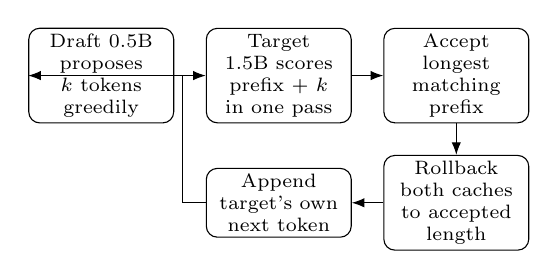
\begin{tikzpicture}[node distance=4mm, box/.style={draw,rounded corners,align=center,font=\scriptsize,minimum height=6.5mm,text width=1.7cm,inner sep=2pt}, arr/.style={-{Latex[length=1.6mm]}}]
\node[box] (d) {Draft 0.5B proposes $k$ tokens greedily};
\node[box,right=of d] (v) {Target 1.5B scores prefix + $k$ in one pass};
\node[box,right=of v] (c) {Accept longest matching prefix};
\node[box,below=of c] (r) {Rollback both caches to accepted length};
\node[box,left=of r] (b) {Append target's own next token};
\draw[arr] (d)--(v); \draw[arr] (v)--(c); \draw[arr] (c)--(r); \draw[arr] (r)--(b);
\draw[arr] (b.west) -- ++(-3mm,0) |- (d.west);
\end{tikzpicture}
}
\caption{Draft, verify and rollback loop of speculative decoding.}
\label{fig:spec}
\end{figure}
\begin{algorithm}[t]
\caption{Greedy speculative decoding}
\label{alg:spec}
\begin{algorithmic}[1]
\Require target $T$, draft $D$ (same tokenizer), prompt $x$, draft length $k$, max new tokens $N$
\State prefill caches of $T$ and $D$ with $x$; $y\gets[\,]$
\While{$|y|<N$ and no EOS}
  \State $d_1..d_k\gets$ greedy decode of $D$ (each step uses $D$'s cache)
  \State $t_0..t_k\gets \arg\max$ of $T$ logits on $[\text{last},d_1..d_k]$ (one pass)
  \State $a\gets$ largest $a\le k$ with $d_i=t_{i-1}$ for all $i\le a$
  \State append $d_1..d_a$ and $t_a$ to $y$
  \State roll back caches of $T$ and $D$ to the verified prefix (discard rejected positions)
\EndWhile
\State \Return $y$
\end{algorithmic}
\end{algorithm}

\subsection{Application workflow}
\label{sec:app}
``Kormat'' is a FastAPI service with a static browser front end. A user pastes a patient description and one or more criteria; the server splits sentences, builds the shared prompt, decodes (with cache and optional speculation), parses and validates the JSON (cited IDs must exist in the note), and returns per-criterion label, cited IDs, evidence text and an explanation based only on the note (Fig.~\ref{fig:app}). Multiple criteria may be combined into a patient--trial summary by explicit rules, which is an aggregation and not a ground-truth outcome. % TODO-INTERPRET: add rule table and screenshots (figures/app_*.png) when TGA-36..41 land.
\begin{figure}[t]\centering
\resizebox{\columnwidth}{!}{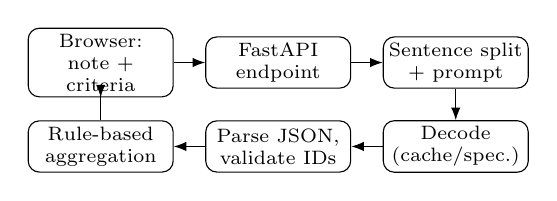
\begin{tikzpicture}[node distance=4mm, box/.style={draw,rounded corners,align=center,font=\scriptsize,minimum height=6.5mm,text width=1.7cm,inner sep=2pt}, arr/.style={-{Latex[length=1.6mm]}}]
\node[box] (u) {Browser: note + criteria};
\node[box,right=of u] (api) {FastAPI endpoint};
\node[box,right=of api] (sp) {Sentence split + prompt};
\node[box,below=of sp] (g) {Decode (cache/spec.)};
\node[box,left=of g] (pa) {Parse JSON, validate IDs};
\node[box,left=of pa] (ag) {Rule-based aggregation};
\draw[arr] (u)--(api); \draw[arr] (api)--(sp); \draw[arr] (sp)--(g); \draw[arr] (g)--(pa); \draw[arr] (pa)--(ag);
\draw[arr] (ag.north) -- ++(0,4mm) -| (u.south);
\end{tikzpicture}
}
\caption{Application request flow.}
\label{fig:app}
\end{figure}

\section{Experimental Setup and Metrics}
\label{sec:setup}
\textbf{Hardware and software.} All reported numbers were produced on a laptop with an Intel Core i5-10310U (4 cores, 8 threads), 15~GB RAM and no GPU, with Python 3.10, PyTorch 2.5.1 (CPU), Transformers 4.46.3 and PEFT 0.13.2, all pinned in the repository lock file. Only one large model is loaded at a time (a file lock enforces this). Each run writes a record (config, environment, metrics) under \texttt{results/<area>/}, and the commit SHA is stored with it.

\textbf{Compared systems.} (i) The base Qwen2.5-1.5B-Instruct with the same prompt contract (\emph{before}); (ii) the base plus the shared LoRA adapter, merged into fp32 weights (\emph{after}; merged and unmerged outputs are identical on our check, $|\Delta\text{logit}|\le5.8\times10^{-5}$). Both are evaluated on identical examples with the same parser and the same decoding: plain greedy (\texttt{do\_sample=False}), at most 48 new tokens, fp32, batch 1, with \texttt{repetition\_penalty=1.0}. That last setting matters. Qwen's \texttt{generation\_config.json} ships a repetition penalty of 1.1 that Hugging Face applies \emph{even in greedy mode}; our first validation pass inherited it unnoticed. We kept that pass as an ablation and re-ran everything with the penalty switched off, which also makes the evaluation decoding identical to our hand-written decoders. Invalid or unparsable outputs are counted as an explicit INVALID class and are never dropped. We tuned no hyperparameters, prompts or thresholds: the prompt is fixed by the adapter's training contract, and the full configuration (model and adapter revisions and hashes, decoding settings) was frozen in \texttt{configs/final.yaml} before the first test access. Because of the deadline, the test runs were executed before the final validation run. This leaks nothing, since nothing is selected on validation. \texttt{results/test\_access.log} records every access to the sealed test split.

\textbf{Classification metrics.} We report accuracy, macro-F1, per-class precision/recall/F1 and confusion matrices, overall and separately for inclusion and exclusion criteria, each over its own four-way label set; the overall view uses the union of the six labels. Labels are never collapsed to binary. Macro-F1 is the unweighted mean over the classes of the label set that occur in the gold labels or the predictions. A class absent from both has undefined F1 and is not counted as zero; the fixed-list variant is stored alongside in the metric files. INVALID predictions count as errors.

\textbf{Evidence metrics.} Let $G$ be the expert sentence-ID set and $P$ the predicted set (IDs not present in the note are removed and counted separately as hallucinated). \emph{Micro} precision/recall/F1 pool $|P\cap G|$, $|P|$ and $|G|$ over all records, so records where both sets are empty contribute nothing. \emph{Macro} averages per-record scores with explicit rules for empty sets:
\begin{itemize}
\item $G=P=\emptyset$ scores $P=R=F_1=1$ (a correct abstention);
\item $G=\emptyset$, $P\neq\emptyset$ scores $P=0$, $R=1$, $F_1=0$;
\item $G\neq\emptyset$, $P=\emptyset$ scores $P=1$, $R=0$, $F_1=0$.
\end{itemize}
We also report the macro average over non-empty-gold records only, and the count of records in each of the four empty/non-empty cells.

\textbf{Systems metrics.} Latency per generated token and end-to-end per criterion (median and spread over repeated runs after warm-up), peak resident memory, speed-up of cache vs.\ recomputation, peak memory and time of tiled vs.\ reference attention across sequence lengths, and for speculative decoding the acceptance rate, mean accepted tokens per verify pass and wall-clock speed-up over target-only greedy decoding. Output equality with the baseline is checked token by token.

\textbf{Uncertainty.} With 8 test patients, metric differences are noisy; we report counts alongside percentages and, where available, 95\% percentile bootstrap intervals (1{,}000 resamples of criteria, seed 42).

\section{Results and Discussion}
\label{sec:results}
% OWNED BY THE RESULTS AUTHOR: this section is a skeleton. Do not invent numbers; every \maybeinput table is generated by the code.
\subsection{Fine-tuning: training curves and validation}
\begin{figure}[t]\centering
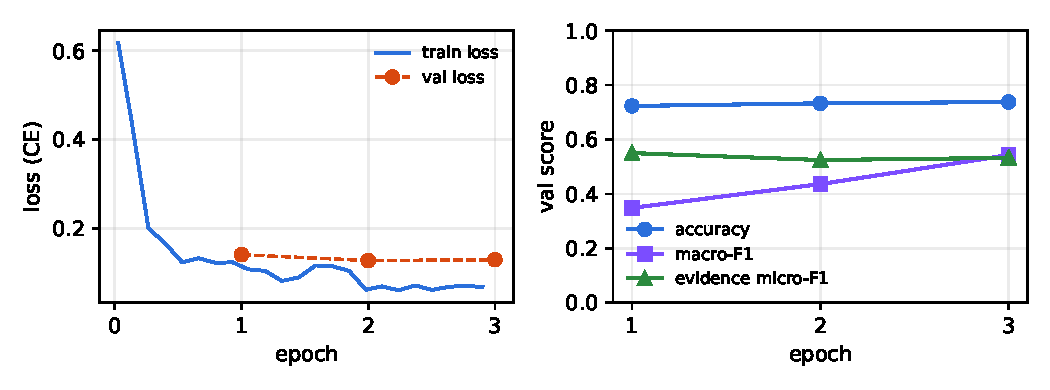
\includegraphics[width=\columnwidth]{figures/training_curves_shared.pdf}
\caption{Logged curves of the shared training run that produced the adapter (joint session, disclosed). Left: training loss per logged optimizer step and validation loss per epoch. Right: per-epoch validation scores computed by that run's own evaluation code, used to select epoch~3. Our independent evaluation is in Table~\ref{tab:cls}.}\label{fig:train}
\end{figure}
Fig.~\ref{fig:train} shows the run that produced the adapter. Its configuration is identical to our \texttt{configs/train.yaml}, and its logs are kept unmodified, with their source, in \texttt{results/finetune/shared\_run/}. The completion-only loss drops from 0.62 to about 0.12 within the first half epoch, then flattens near 0.06--0.07. Validation loss is lowest after epoch~2 (0.127) and almost unchanged after epoch~3 (0.129), so there is no sign of strong overfitting over three epochs on 602 examples. The run selected epoch~3 by validation macro-F1, which keeps rising (0.35, 0.44, 0.54) while accuracy is nearly flat (0.72--0.74). That pattern means the later epochs mainly improve the rare classes. These per-epoch numbers come from the training run's own evaluation and are \emph{not} our results. Our own code (\texttt{configs/train.yaml}, \texttt{src/kormat/finetune/train.py}) reproduces the configuration and was verified end to end only by a CPU smoke run on Qwen2.5-0.5B (loss 0.52$\rightarrow$0.12 over 30 steps, adapter saved and reloaded; \texttt{results/finetune/smoke/}).
\maybeinput{tables/finetune_summary}

\subsection{Before/after on identical examples}
\maybeinput{tables/eval_before_after}
% TODO-INTERPRET: accuracy and macro-F1 change, per-class changes, inclusion vs exclusion, INVALID rate before/after.

\subsection{Evidence retrieval}
\maybeinput{tables/evidence_prf}
% TODO-INTERPRET: P/R/F1, treatment of empty-gold records.

\subsection{Error analysis}
\maybeinput{tables/error_cases}
On the test split the fine-tuned model made 55 label errors out of 206. Another 33 criteria had the right label but a different evidence set: in 19 the model cited sentences outside the expert set, in 17 it missed expert sentences, and some did both. No output was unparsable, and no cited ID was outside the note. Table~\ref{tab:errors} traces eleven distinct cases; the full list with sentence text is in \texttt{docs/research/error\_analysis.md}. Four patterns emerge.

\textbf{(A) Absence treated as proof (28 errors).} \emph{Every} exclusion criterion whose expert label is ``not enough information'' was predicted ``not excluded''. When no sentence mentions the excluding condition (e.g.\ eGFR, prior axillary surgery), the model concludes the patient is not excluded, which is exactly the inference the task forbids. The training data explain the shortcut: 292 of the 388 training exclusion criteria are ``not excluded'', 218 of them without any evidence sentence, against only 65 ``not enough information''. \textbf{(B)} Nine ``not applicable'' exclusions collapse to the same default. Together, A and B make up 37 of the 55 errors and drive exclusion macro-F1 down. For a screening aid this is the unsafe direction, because missing information is hidden rather than flagged.

\textbf{(C) Over-abstention on inferable facts (14).} The opposite failure appears on inclusion criteria that need clinical inference: blood pressure 80/60 with tachycardia means shock (case 185), and an acute femoral complication rules out an elective endarterectomy (161). Case 162 is \emph{contradictory}: the note describes a different vascular problem than the criterion. In several of these cases the model cites the right sentences but abstains. Its evidence localisation is therefore better than its judgement, so the explanation still directs the reviewer to the relevant text. Case 196 is a plain \emph{missing-information} false alarm: the age is stated, but the model misses it. \textbf{(D)} Four errors confuse ``not applicable'' with ``not enough information'' on conditional, sex-specific criteria, where expert conventions themselves vary (case 322).

\textbf{Implication.} A cheap deterministic guard, downgrading an exclusion ``not excluded'' with \emph{empty} evidence to ``not enough information'', would target pattern A without retraining. Rebalancing the exclusion labels during training is the principled fix. We did not apply either to the reported numbers.

\subsection{KV cache}
\maybeinput{tables/kvcache}
\begin{figure}[t]\centering
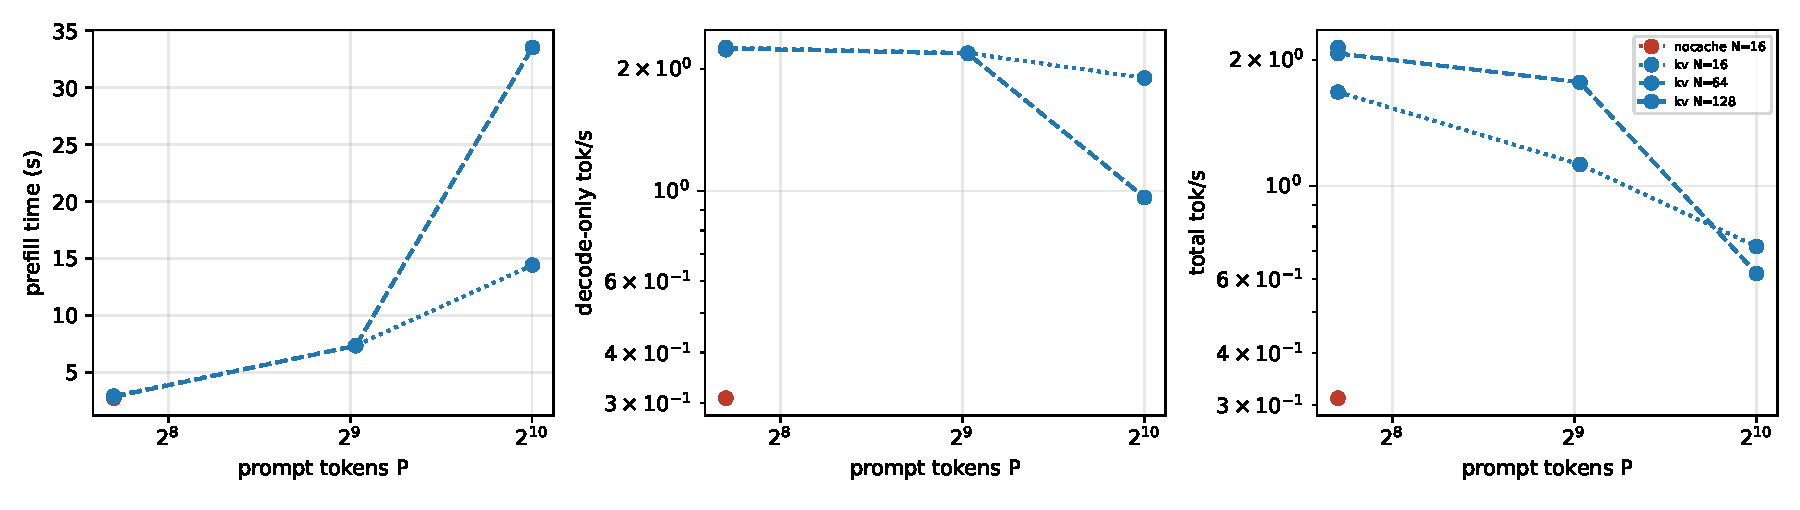
\includegraphics[width=\columnwidth]{figures/kv_speed.pdf}
\caption{Decode throughput of the merged fine-tuned 1.5B model on the CPU, with our pre-allocated KV cache and with the no-cache reference, as a function of prompt length (median of 3 timed runs after 1 warm-up).}\label{fig:kvspeed}
\end{figure}
\textbf{Correctness.} Table~\ref{tab:kveq} shows that the cache-aware decoder reproduces the uncached reference token for token in all five tested input/output combinations ($P\in\{208,523,1025\}$ prompt tokens, $N$ up to 128 new tokens) in fp32. The first-step logits are bit-identical ($\Delta=0$), because both paths run the same prefill. Later steps differ by at most $1.2\times10^{-4}$, which comes from the different reduction order of a $1\times d$ versus a $(P{+}t)\times d$ matrix product, and is far below the top-1/top-2 margin, so no argmax flipped. Our own \texttt{Cache} subclass is provably on the path: a unit test counts its \texttt{update()} calls, and deliberately shifting the position ids breaks equivalence, so the test is not vacuous.

\textbf{Speed.} Table~\ref{tab:kv} and Fig.~\ref{fig:kvspeed} show the asymptotic difference. Without a cache, every new token re-encodes the whole sequence, so decode throughput falls with prompt length (0.31, 0.13 and 0.07 tok/s at $P=208$, 523 and 1025). With the cache, each step processes one token against stored keys and values, and throughput stays roughly flat (2.26, 2.19 and 1.90 tok/s). The measured speed-up therefore grows from $7\times$ to about $17\times$ and $27\times$; the last two compare per-token decode rates measured at different $N$, because the no-cache grid was capped at small $N$ to fit the time budget. Prefill time is the same in both modes (about 2.9\,s at $P=208$), since it is a single forward pass either way.

\textbf{Memory.} Thanks to grouped-query attention (2 KV heads), the analytical cache is only 28\,KB per token in fp32 (12--60\,MB here). That is negligible next to the 6.3\,GB of fp32 weights, so peak RSS barely moves (6.35 to 6.54\,GB). On this hardware the cache trades a few megabytes for an order-of-magnitude speed-up. One outlier ($P=1025$, $N=64$: 0.97 tok/s) was measured while other jobs shared the CPU and is treated as noise.

\textbf{Prefix reuse in evaluation.} The evaluation runner applies the same mechanism across criteria. The system prompt and patient note (273 tokens in the checked example) are prefilled once per patient, and the cache is copied for each criterion. Outputs were token-identical to plain generation (3/3, Table~\ref{tab:prefix}). Per-criterion latency fell from 10.7\,s to 7.2\,s when the prefix was reused, but the mean gain was only about $1.2\times$, because decoding the roughly 15-token answer, not the prompt, dominates on a CPU.
\maybeinput{tables/prefix_cache}

\subsection{Tiled attention}
\maybeinput{tables/attention}
\begin{figure}[t]\centering
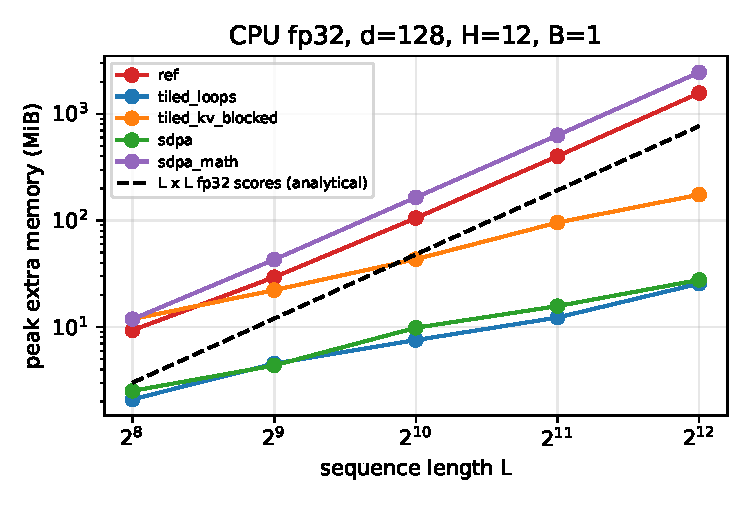
\includegraphics[width=\columnwidth]{figures/attn_memory_vs_L.pdf}
\caption{Peak extra memory of one attention call versus sequence length ($d=128$, 12 heads, fp32, CPU). The reference and the math backend materialise the $L\times L$ score matrix; tiled attention does not.}\label{fig:attnmem}
\end{figure}
\textbf{Correctness.} Across 1{,}680 validation cases (lengths 1 to 1024 including non-multiples of the block size, $L_q\neq L_k$ decode and verify shapes, GQA, causal, padding and fully masked rows, and four block sizes), the tiled online-softmax kernel matches a float64 ground truth within the stated tolerances in every case (Table~\ref{tab:attnval}; timings in Table~\ref{tab:attnbench}). The maximum absolute error is $2.5\times10^{-6}$ in fp32, $9.7\times10^{-4}$ in fp16 and $7.8\times10^{-3}$ in bf16; bf16 needs a relative tolerance of $8\times10^{-3}$ because its unit round-off is $2^{-8}$. A stability test multiplies the logits by 1000: a naive softmax returns NaN, while the running-max formulation stays finite. Routing the attention of a small Qwen2 model through our kernel gives identical greedy tokens (max logit difference about $2\times10^{-7}$).

\textbf{Speed and memory.} The memory advantage is real but the speed advantage is not (Fig.~\ref{fig:attnmem}). At $L=4096$, the reference needs 1.57\,GB of extra memory, close to the 0.77\,GB analytical size of the fp32 score matrix plus the softmax copy, whereas the loop-tiled version needs 26\,MB. Its run time, however, is 5.0\,s against 3.0\,s for the reference and 1.9\,s for PyTorch's fused CPU kernel. This is expected for educational PyTorch code. Each tile launches several separate operators (matmul, max, exp, sum, rescale), each reading and writing main memory. Nothing is fused, and Python loop overhead grows with the number of tiles: run time falls from 8.0\,s at block 16 to 0.6\,s at block 256 for $L=2048$. FlashAttention's speed comes from keeping tiles in on-chip SRAM inside one fused kernel, which plain PyTorch cannot express. On this CPU, therefore, tiling buys linear memory, not speed.

\subsection{Speculative decoding}
\maybeinput{tables/speculative}
\begin{figure}[t]\centering
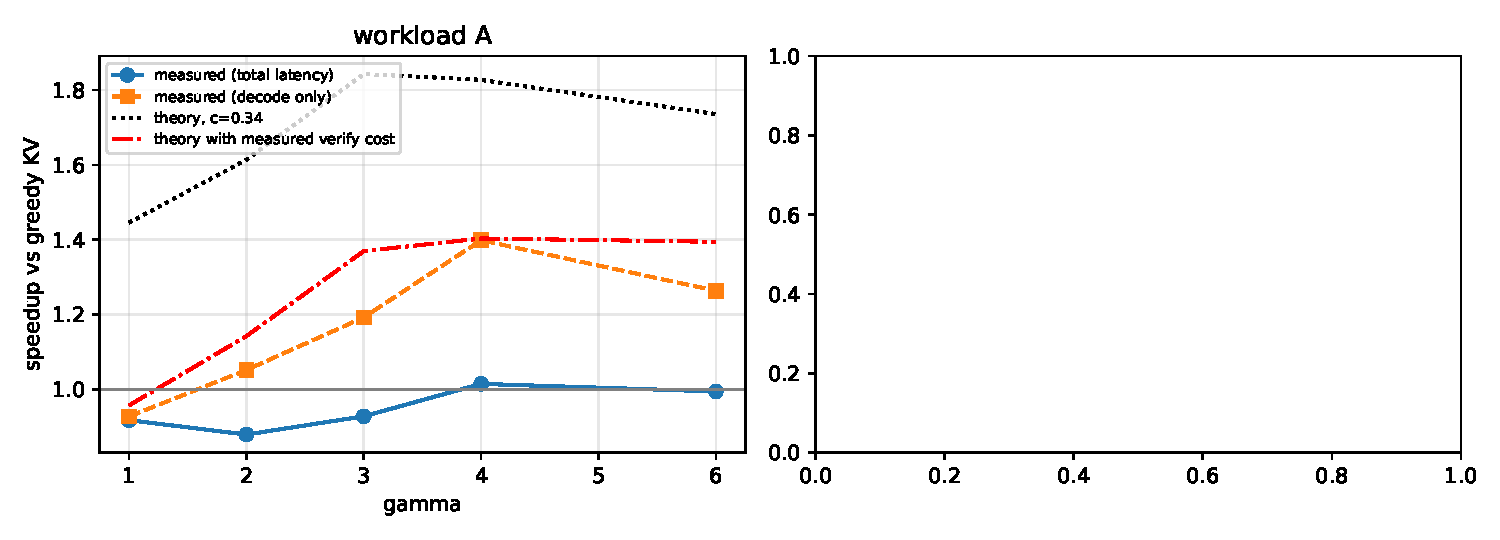
\includegraphics[width=\columnwidth]{figures/spec_speedup.pdf}
\caption{Measured speculative speed-up versus draft length $\gamma$, against the theoretical curve with the measured draft/target cost ratio $c=0.337$, and with the measured verification cost.}\label{fig:spec}
\end{figure}
\textbf{Correctness.} Our draft--verify--rollback decoder produced exactly the target's greedy sequence in 18 of 18 runs on validation prompts ($\gamma\in\{2,4,8\}$), and in every benchmark run (Tables~\ref{tab:speceq} and~\ref{tab:specbench}). The cache invariant (both caches hold exactly the committed prefix) is asserted after every round. Unit tests cover rejection at the first token, full acceptance with the bonus token, EOS inside an accepted block, and overshooting \texttt{max\_new\_tokens}.

\textbf{Efficiency.} The 0.5B draft agrees with the target often: the acceptance rate is 0.73 to 0.93 depending on $\gamma$. Even so, the end-to-end speed-up is between $0.88\times$ and $1.01\times$, i.e.\ no gain. Fig.~\ref{fig:spec} explains why with three measured effects.
\begin{enumerate}
\item The draft is not cheap enough. One draft step costs $c=0.337$ of a target step (146 vs 434\,ms), whereas the analysis of Leviathan et al. assumes $c\ll1$.
\item Verification is not free. Scoring 2 to 9 tokens in one target pass took 731 to 764\,ms, about $1.7\times$ a single decode step, because on a CPU the extra rows of the 151k-vocabulary output projection and the attention cost real FLOPs. A GPU at batch 1 would be memory-bound instead, and that cost would vanish.
\item Our answers are short, about 15 tokens. Prefill of both models (about 9\,s) dominates the end-to-end time, so even the 1.40$\times$ decode-only gain at $\gamma=4$ is diluted to about 1.0$\times$.
\end{enumerate}
With $\alpha\approx0.83$ and $\gamma=4$, the theory predicts $1.5\times$ with $c$ alone and about $1.2\times$ once the measured verification cost is included, in line with the measured decode-only speed-up. Speculative decoding would pay off for longer outputs and on hardware where verifying several tokens costs about as much as decoding one.

\subsection{Application}
\begin{figure}[t]\centering
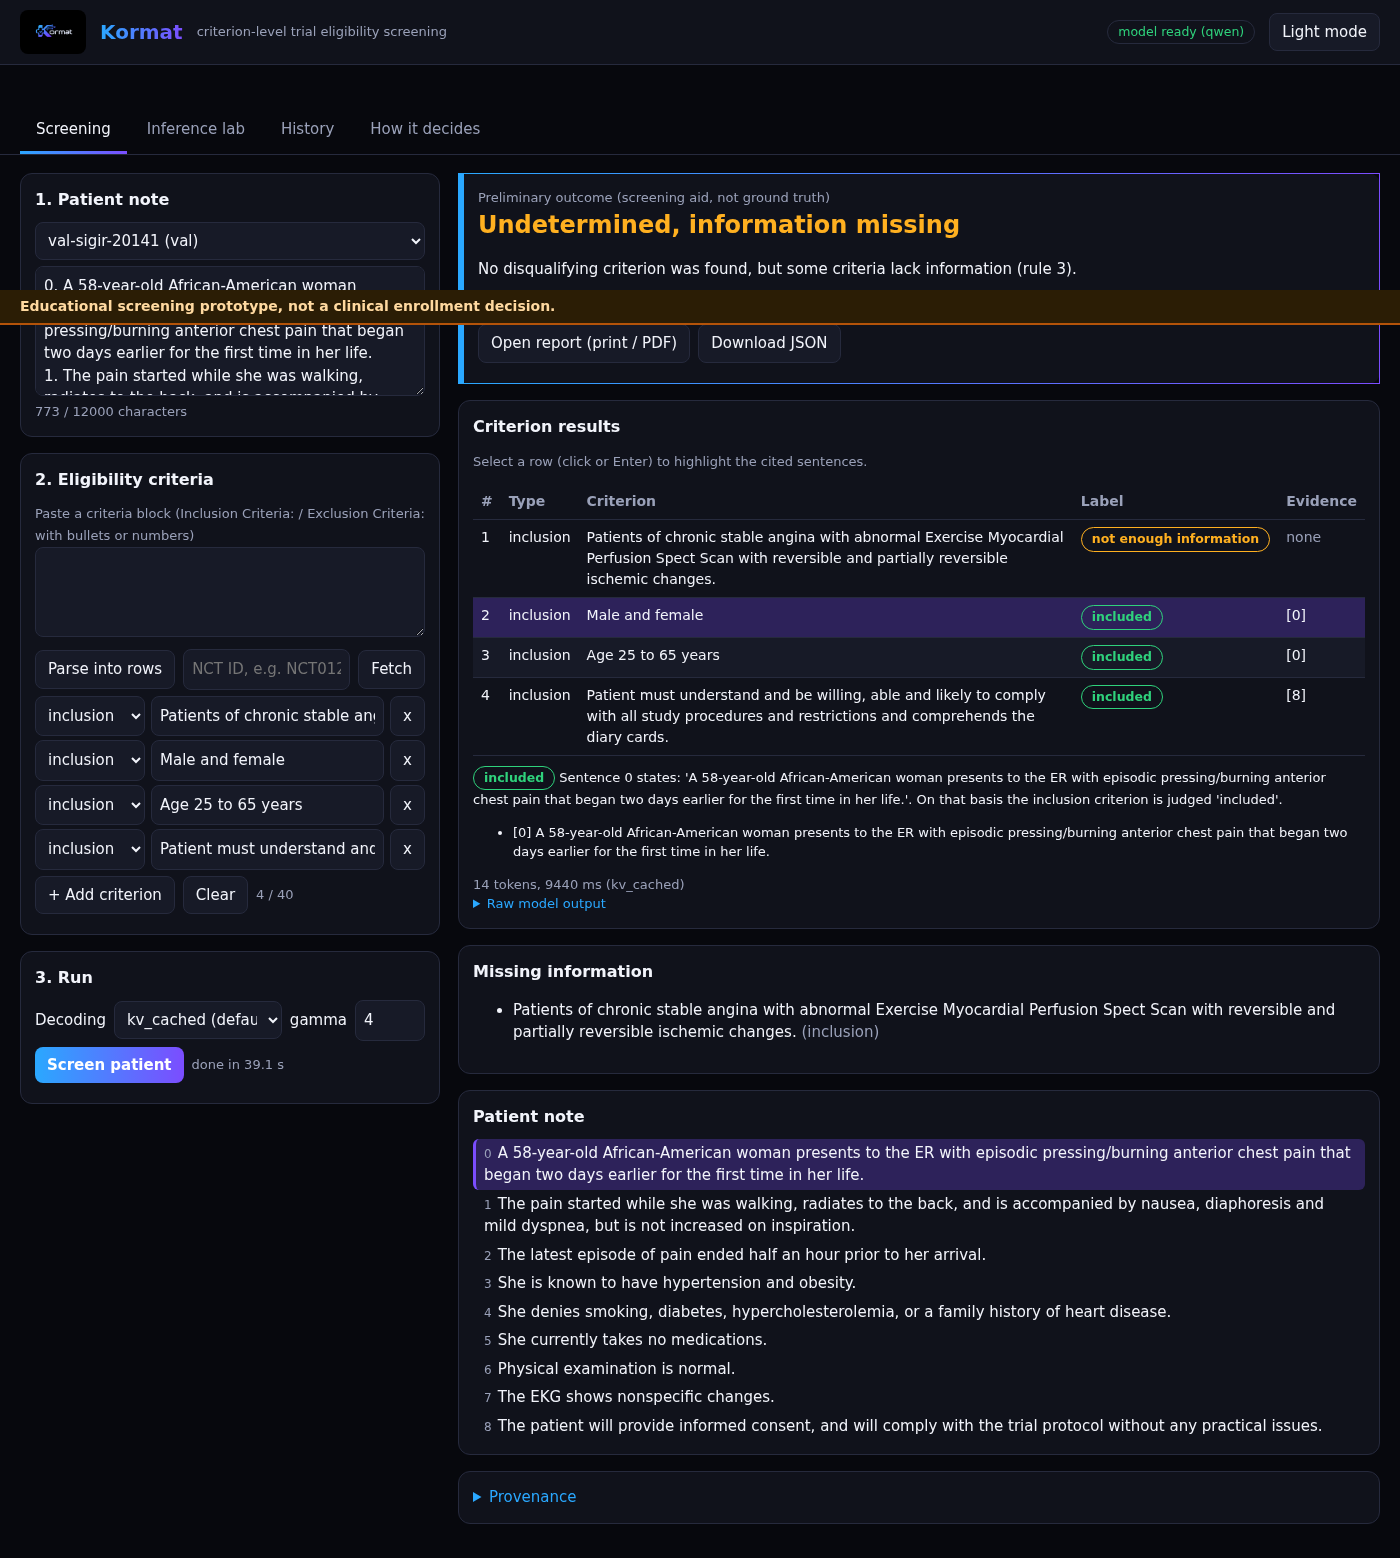
\includegraphics[width=\columnwidth]{figures/app_real_results.png}
\caption{Kormat screening a validation patient with the fine-tuned model (real engine, KV-cached decoding). The second criterion is selected and its cited sentence~0 is highlighted in the numbered note. The missing-information list and the rule-based preliminary outcome are shown, together with the disclaimer banner.}\label{fig:app}
\end{figure}
\begin{figure}[t]\centering
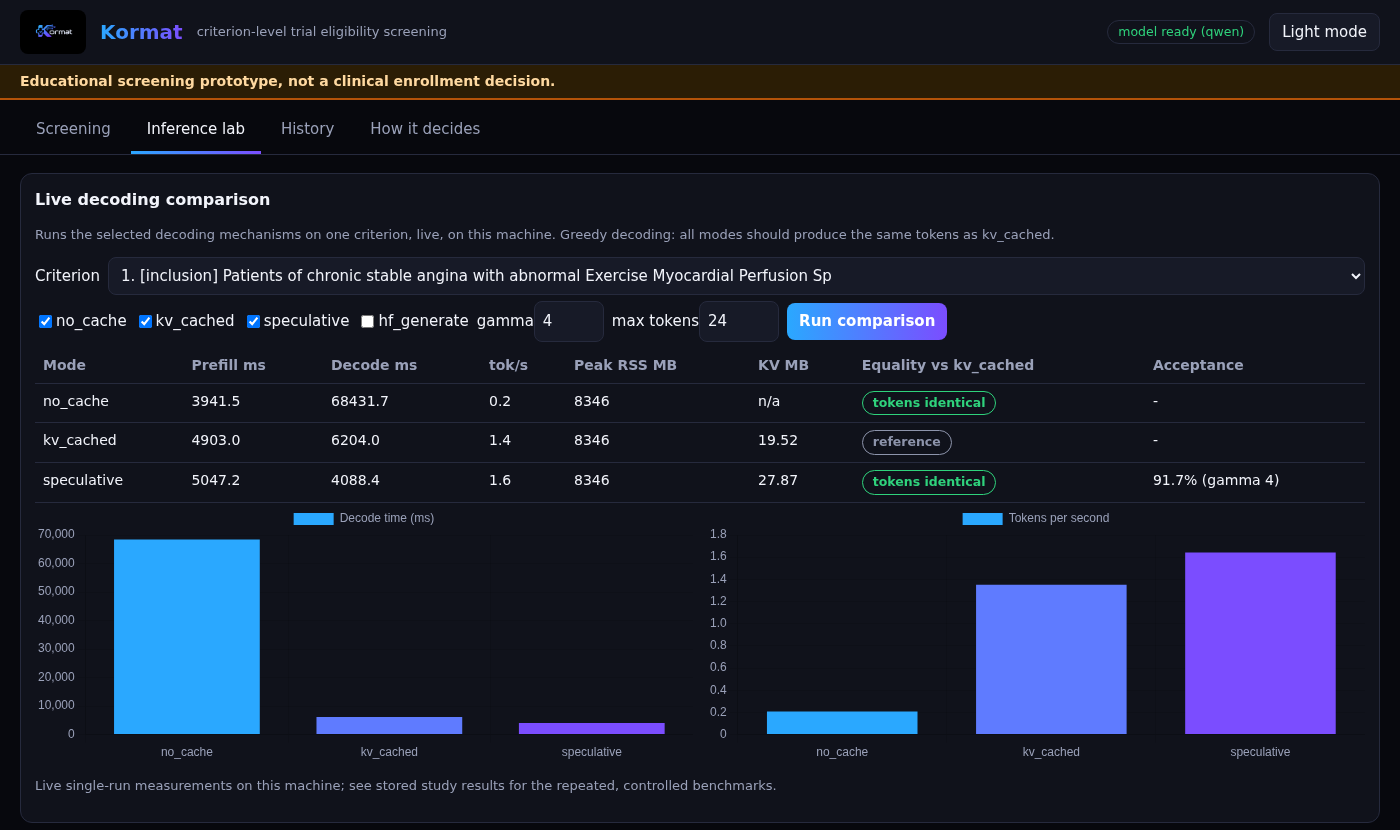
\includegraphics[width=\columnwidth]{figures/app_real_lab.png}
\caption{Inference lab: the same criterion decoded live with no cache, our KV cache and speculative decoding ($\gamma=4$). The lab shows timings, memory, acceptance rate and token equality against the KV-cached reference.}\label{fig:lab}
\end{figure}
Fig.~\ref{fig:app} shows the screening workflow on the real fine-tuned model. A user pastes a note (free text is split into numbered sentences), enters or pastes the criteria (or fetches them by NCT ID), and runs the screen. Each criterion row shows the label, the cited IDs and an explanation quoted only from those sentences, and clicking a row highlights the evidence. In a recorded real-engine session (\texttt{results/app/*/real\_smoke.json}), with the evaluation running concurrently on the same CPU, the model loaded in 15\,s from the local cache. Each criterion took 9.5--10.4\,s, and all four criteria of the sample patient matched the expert labels. The patient--trial outcome is an explicit rule (any exclusion met or inclusion unmet $\Rightarrow$ likely ineligible; otherwise any missing information $\Rightarrow$ undetermined; otherwise potentially eligible). The app presents it as a preliminary aggregation, never as ground truth.

The lab (Fig.~\ref{fig:lab}) re-runs any criterion live under each decoding mode. For a 24-token output, no-cache decoding took 68.9\,s, KV-cached decoding 6.2\,s and speculative decoding 4.0\,s, with an acceptance rate of 91.7\%. All three produced the same tokens, which the lab confirms with an equality badge. On this longer output speculative decoding did help, consistent with the analysis above: the gain appears once decoding, not prefill, dominates. Invalid inputs (empty note, too many criteria, malformed criteria, the model still loading, an offline NCT fetch) return explanatory messages and the app keeps working; the automated tests cover each case. Reports export as print-ready HTML and JSON with provenance (model and adapter revision, adapter hash, git commit, decoding settings) and persist across restarts.

\section{Limitations}
\label{sec:limits}
\begin{itemize}
\item \textbf{Small data.} 53 patients, 8 in test; confidence intervals are wide and per-class results for rare labels rest on few examples.
\item \textbf{Shared adapter.} The adapter was trained in a joint GPU session; we neither re-trained it independently nor ran seeds or ablations of the training, so we cannot separate training-recipe effects from base-model effects. Our own training script is shown to run end to end only on a short CPU smoke run with the 0.5B model. The other candidate models were compared by configuration arithmetic only.
\item \textbf{Criterion-level labels only.} The dataset has no patient--trial ground truth; our aggregation is rule based and unvalidated against experts.
\item \textbf{Length handling.} In this dataset the longest prompt plus target is 622 tokens, so with a 1{,}024-token budget no example was truncated and no gold evidence was lost. Unseen notes in the application can be much longer; our policy then drops whole sentences, which could remove evidence. The app warns the user when this happens.
\item \textbf{CPU-only evaluation.} Generation on a 4-core laptop CPU takes about 8\,s per criterion, which ruled out repeated evaluation runs. Some systems benchmarks were run on reduced grids (e.g.\ the no-cache path only up to 64 new tokens) and with 3 repeats, and some timings were taken while other jobs shared the CPU.
\item \textbf{Decoding pitfall.} Our first validation pass silently inherited a repetition penalty from the model's default generation configuration. We caught it and re-ran, but it shows how library defaults can change ``greedy'' results.
\item \textbf{CPU-specific systems results.} Tiled attention and speculative decoding are known GPU-driven speed-ups; our timings are for one laptop CPU with eager PyTorch and do not generalise to GPUs or other CPUs.
\item \textbf{Not clinical software.} The system is a research prototype; outputs must not be used for real patient decisions.
\end{itemize}

\section{Conclusion}
\label{sec:conclusion}
We built an open, locally runnable criterion-level eligibility screener around a LoRA-adapted Qwen2.5-1.5B-Instruct, evaluated it against its unadapted base on identical held-out patients, and implemented our own KV-cache decoder, tiled attention and speculative decoder with measurements on a CPU. \todo{one-sentence headline result and one-sentence systems finding, after Results are final.} Future work: independent multi-seed training, larger external evaluation, and GPU benchmarks of the same code.


\section*{Availability}
Source code: \todo{GitHub URL (TahaGPT/Kormat)}. Adapter weights: Hugging Face \texttt{arceus1rk/eligitrace-qwen2.5-1.5b-lora}. Split manifest and logs are in the repository under \texttt{results/}. Demo video: \todo{video link}.

\bibliographystyle{IEEEtran}
\bibliography{refs}

\appendices
\section{Use of AI Tools}
\label{app:ai}
\textbf{Tools.} This project was planned, coded and drafted with Claude Code (a lead agent, Claude Opus 5.5, coordinating specialist agents running Claude Sonnet 5.5) working in the repository under the author's direction. AI assistance covered task planning, literature search and drafting, source code, tests, the web application, LaTeX and figure scripts.

\textbf{Verification.} Every bibliographic entry was opened on its arXiv, publisher or Crossref page before inclusion; model facts come from the Hugging Face \texttt{config.json} files and model cards; all reported numbers are produced by scripts that write run records with the commit SHA, not typed by hand; implementations are checked against reference ones (attention against softmax attention, speculative output against greedy output) by tests; the split is checked for patient leakage. \todo{the author states which outputs they personally reviewed, ran and can explain.}

\textbf{Joint training disclosure.} The LoRA adapter (\texttt{arceus1rk/eligitrace-qwen2.5-1.5b-lora}) was trained in a joint session on a shared GPU with M.\ Ruhan Kamran (23i-0062), because the author's laptop has no GPU. It is a disclosed shared artefact. No code, results, figures or text were copied from the other student's repository.

\textbf{Limits of AI use.} AI-generated text and code may contain errors; claims in this report are limited to what the cited sources and our measurements support.


\end{document}
